% Options for packages loaded elsewhere
\PassOptionsToPackage{unicode}{hyperref}
\PassOptionsToPackage{hyphens}{url}
%
\documentclass[
]{article}
\usepackage{amsmath,amssymb}
\usepackage{lmodern}
\usepackage{iftex}
\ifPDFTeX
  \usepackage[T1]{fontenc}
  \usepackage[utf8]{inputenc}
  \usepackage{textcomp} % provide euro and other symbols
\else % if luatex or xetex
  \usepackage{unicode-math}
  \defaultfontfeatures{Scale=MatchLowercase}
  \defaultfontfeatures[\rmfamily]{Ligatures=TeX,Scale=1}
\fi
% Use upquote if available, for straight quotes in verbatim environments
\IfFileExists{upquote.sty}{\usepackage{upquote}}{}
\IfFileExists{microtype.sty}{% use microtype if available
  \usepackage[]{microtype}
  \UseMicrotypeSet[protrusion]{basicmath} % disable protrusion for tt fonts
}{}
\makeatletter
\@ifundefined{KOMAClassName}{% if non-KOMA class
  \IfFileExists{parskip.sty}{%
    \usepackage{parskip}
  }{% else
    \setlength{\parindent}{0pt}
    \setlength{\parskip}{6pt plus 2pt minus 1pt}}
}{% if KOMA class
  \KOMAoptions{parskip=half}}
\makeatother
\usepackage{xcolor}
\usepackage[margin=1in]{geometry}
\usepackage{color}
\usepackage{fancyvrb}
\newcommand{\VerbBar}{|}
\newcommand{\VERB}{\Verb[commandchars=\\\{\}]}
\DefineVerbatimEnvironment{Highlighting}{Verbatim}{commandchars=\\\{\}}
% Add ',fontsize=\small' for more characters per line
\usepackage{framed}
\definecolor{shadecolor}{RGB}{248,248,248}
\newenvironment{Shaded}{\begin{snugshade}}{\end{snugshade}}
\newcommand{\AlertTok}[1]{\textcolor[rgb]{0.94,0.16,0.16}{#1}}
\newcommand{\AnnotationTok}[1]{\textcolor[rgb]{0.56,0.35,0.01}{\textbf{\textit{#1}}}}
\newcommand{\AttributeTok}[1]{\textcolor[rgb]{0.77,0.63,0.00}{#1}}
\newcommand{\BaseNTok}[1]{\textcolor[rgb]{0.00,0.00,0.81}{#1}}
\newcommand{\BuiltInTok}[1]{#1}
\newcommand{\CharTok}[1]{\textcolor[rgb]{0.31,0.60,0.02}{#1}}
\newcommand{\CommentTok}[1]{\textcolor[rgb]{0.56,0.35,0.01}{\textit{#1}}}
\newcommand{\CommentVarTok}[1]{\textcolor[rgb]{0.56,0.35,0.01}{\textbf{\textit{#1}}}}
\newcommand{\ConstantTok}[1]{\textcolor[rgb]{0.00,0.00,0.00}{#1}}
\newcommand{\ControlFlowTok}[1]{\textcolor[rgb]{0.13,0.29,0.53}{\textbf{#1}}}
\newcommand{\DataTypeTok}[1]{\textcolor[rgb]{0.13,0.29,0.53}{#1}}
\newcommand{\DecValTok}[1]{\textcolor[rgb]{0.00,0.00,0.81}{#1}}
\newcommand{\DocumentationTok}[1]{\textcolor[rgb]{0.56,0.35,0.01}{\textbf{\textit{#1}}}}
\newcommand{\ErrorTok}[1]{\textcolor[rgb]{0.64,0.00,0.00}{\textbf{#1}}}
\newcommand{\ExtensionTok}[1]{#1}
\newcommand{\FloatTok}[1]{\textcolor[rgb]{0.00,0.00,0.81}{#1}}
\newcommand{\FunctionTok}[1]{\textcolor[rgb]{0.00,0.00,0.00}{#1}}
\newcommand{\ImportTok}[1]{#1}
\newcommand{\InformationTok}[1]{\textcolor[rgb]{0.56,0.35,0.01}{\textbf{\textit{#1}}}}
\newcommand{\KeywordTok}[1]{\textcolor[rgb]{0.13,0.29,0.53}{\textbf{#1}}}
\newcommand{\NormalTok}[1]{#1}
\newcommand{\OperatorTok}[1]{\textcolor[rgb]{0.81,0.36,0.00}{\textbf{#1}}}
\newcommand{\OtherTok}[1]{\textcolor[rgb]{0.56,0.35,0.01}{#1}}
\newcommand{\PreprocessorTok}[1]{\textcolor[rgb]{0.56,0.35,0.01}{\textit{#1}}}
\newcommand{\RegionMarkerTok}[1]{#1}
\newcommand{\SpecialCharTok}[1]{\textcolor[rgb]{0.00,0.00,0.00}{#1}}
\newcommand{\SpecialStringTok}[1]{\textcolor[rgb]{0.31,0.60,0.02}{#1}}
\newcommand{\StringTok}[1]{\textcolor[rgb]{0.31,0.60,0.02}{#1}}
\newcommand{\VariableTok}[1]{\textcolor[rgb]{0.00,0.00,0.00}{#1}}
\newcommand{\VerbatimStringTok}[1]{\textcolor[rgb]{0.31,0.60,0.02}{#1}}
\newcommand{\WarningTok}[1]{\textcolor[rgb]{0.56,0.35,0.01}{\textbf{\textit{#1}}}}
\usepackage{graphicx}
\makeatletter
\def\maxwidth{\ifdim\Gin@nat@width>\linewidth\linewidth\else\Gin@nat@width\fi}
\def\maxheight{\ifdim\Gin@nat@height>\textheight\textheight\else\Gin@nat@height\fi}
\makeatother
% Scale images if necessary, so that they will not overflow the page
% margins by default, and it is still possible to overwrite the defaults
% using explicit options in \includegraphics[width, height, ...]{}
\setkeys{Gin}{width=\maxwidth,height=\maxheight,keepaspectratio}
% Set default figure placement to htbp
\makeatletter
\def\fps@figure{htbp}
\makeatother
\setlength{\emergencystretch}{3em} % prevent overfull lines
\providecommand{\tightlist}{%
  \setlength{\itemsep}{0pt}\setlength{\parskip}{0pt}}
\setcounter{secnumdepth}{-\maxdimen} % remove section numbering
\ifLuaTeX
  \usepackage{selnolig}  % disable illegal ligatures
\fi
\IfFileExists{bookmark.sty}{\usepackage{bookmark}}{\usepackage{hyperref}}
\IfFileExists{xurl.sty}{\usepackage{xurl}}{} % add URL line breaks if available
\urlstyle{same} % disable monospaced font for URLs
\hypersetup{
  hidelinks,
  pdfcreator={LaTeX via pandoc}}

\author{}
\date{\vspace{-2.5em}}

\begin{document}

\hypertarget{anuxe1lisis-preliminar}{%
\section{Análisis preliminar}\label{anuxe1lisis-preliminar}}

A continuación realizamos un análisis preliminar del dataset de precios
de pañales obtenido. Dividiremos el análisis en las siguientes fases:

\begin{itemize}
\tightlist
\item
  Descripción de atributos
\item
  Consumo de Pañales VS Canásta Básica (Indec)
\item
  Presupuesto destinado a pañales en los primeros \emph{n} meses de vida
  del bebe
\end{itemize}

\begin{Shaded}
\begin{Highlighting}[]
\ImportTok{import}\NormalTok{ pandas }\ImportTok{as}\NormalTok{ pd}
\ImportTok{from}\NormalTok{ matplotlib }\ImportTok{import}\NormalTok{ pyplot }\ImportTok{as}\NormalTok{ plt}
\ImportTok{import}\NormalTok{ seaborn }\ImportTok{as}\NormalTok{ sns}

\NormalTok{sns.}\BuiltInTok{set}\NormalTok{(style}\OperatorTok{=}\StringTok{"darkgrid"}\NormalTok{)}
\KeywordTok{def}\NormalTok{ prepare\_df():}
\NormalTok{    df }\OperatorTok{=}\NormalTok{ pd.read\_csv(}\StringTok{\textquotesingle{}diapers.csv\textquotesingle{}}\NormalTok{)}
    \CommentTok{\# filter items that are wrongly calculated}
    \ControlFlowTok{return}\NormalTok{ df[df[}\StringTok{\textquotesingle{}unit\_price\textquotesingle{}}\NormalTok{] }\OperatorTok{\textless{}} \DecValTok{200}\NormalTok{]}

\NormalTok{df }\OperatorTok{=}\NormalTok{ prepare\_df()}
\NormalTok{df}
\end{Highlighting}
\end{Shaded}

price

website

brand

size

target\_kg\_min

target\_kg\_max

units

unit\_price

0

999.99

www.perfumeriasmiriam.com.ar

babysec

g

8.5

12.0

36

27.78

1

999.99

www.perfumeriasmiriam.com.ar

babysec

m

5.0

9.5

44

22.73

2

999.99

www.perfumeriasmiriam.com.ar

babysec

xxg

13.0

20.0

26

38.46

3

999.99

www.perfumeriasmiriam.com.ar

babysec

xg

11.0

15.0

28

35.71

4

1000.00

www.perfumeriasmiriam.com.ar

pampers

p

5.0

7.5

36

27.78

\ldots{}

\ldots{}

\ldots{}

\ldots{}

\ldots{}

\ldots{}

\ldots{}

\ldots{}

\ldots{}

5345

2230.53

www.anaperfumeriaonline.com.ar

pampers

g

9.0

12.0

68

32.80

5346

4610.42

www.anaperfumeriaonline.com.ar

pampers

xxg

14.0

20.0

88

52.39

5347

4610.42

www.anaperfumeriaonline.com.ar

pampers

xg

12.0

15.0

96

48.03

5348

4610.42

www.anaperfumeriaonline.com.ar

pampers

g

9.0

12.0

110

41.91

5349

557.79

www.anaperfumeriaonline.com.ar

pampers

m

6.0

9.5

18

30.99

5335 rows × 8 columns

\hypertarget{descripciuxf3n-de-atributos}{%
\subsection{Descripción de
atributos}\label{descripciuxf3n-de-atributos}}

Observamos los atributos recabados:

\begin{itemize}
\tightlist
\item
  \textbf{price}. Precio por paquete (antes precio).
\item
  \textbf{website}. Identificar el vendedor.
\item
  \textbf{brand}. Identificar la marca. Extraer atributo de description.
\item
  \textbf{size}. Talle del pañal. Extraer atributo de description.
\item
  \textbf{target\_kg(\_min\textbar\_max)}. Tamaño mínimo y máximo en KGs
  soportado. Clasificar atributo en base a tabla.
\item
  \textbf{units}. Unidades por paquete. Extraer atributo de description.
\item
  \textbf{unit\_price}. Precio unitario. Calcular a partir de
  price/units.
\end{itemize}

\begin{Shaded}
\begin{Highlighting}[]
\NormalTok{df.head()}
\end{Highlighting}
\end{Shaded}

price

website

brand

size

target\_kg\_min

target\_kg\_max

units

unit\_price

0

999.99

www.perfumeriasmiriam.com.ar

babysec

g

8.5

12.0

36

27.78

1

999.99

www.perfumeriasmiriam.com.ar

babysec

m

5.0

9.5

44

22.73

2

999.99

www.perfumeriasmiriam.com.ar

babysec

xxg

13.0

20.0

26

38.46

3

999.99

www.perfumeriasmiriam.com.ar

babysec

xg

11.0

15.0

28

35.71

4

1000.00

www.perfumeriasmiriam.com.ar

pampers

p

5.0

7.5

36

27.78

\begin{Shaded}
\begin{Highlighting}[]
\KeywordTok{def}\NormalTok{ add\_values(ax, feature):}
\NormalTok{    total }\OperatorTok{=} \BuiltInTok{len}\NormalTok{(feature)}
    \ControlFlowTok{for}\NormalTok{ p }\KeywordTok{in}\NormalTok{ ax.patches:}
\NormalTok{        percentage }\OperatorTok{=} \StringTok{\textquotesingle{}}\SpecialCharTok{\{:.1f\}}\StringTok{\%\textquotesingle{}}\NormalTok{.}\BuiltInTok{format}\NormalTok{(}\DecValTok{100} \OperatorTok{*}\NormalTok{ p.get\_height()}\OperatorTok{/}\NormalTok{total)}
\NormalTok{        x }\OperatorTok{=}\NormalTok{ p.get\_x() }\OperatorTok{+}\NormalTok{ p.get\_width() }\OperatorTok{/} \DecValTok{2} \OperatorTok{{-}} \FloatTok{0.2}
\NormalTok{        y }\OperatorTok{=}\NormalTok{ p.get\_y() }\OperatorTok{+}\NormalTok{ p.get\_height()}
\NormalTok{        ax.annotate(percentage, (x, y), size }\OperatorTok{=} \DecValTok{12}\NormalTok{)}

\NormalTok{ax }\OperatorTok{=}\NormalTok{ sns.countplot(y}\OperatorTok{=}\StringTok{"website"}\NormalTok{, data}\OperatorTok{=}\NormalTok{df, orient}\OperatorTok{=}\StringTok{"h"}\NormalTok{)}
\end{Highlighting}
\end{Shaded}

\begin{figure}
\centering
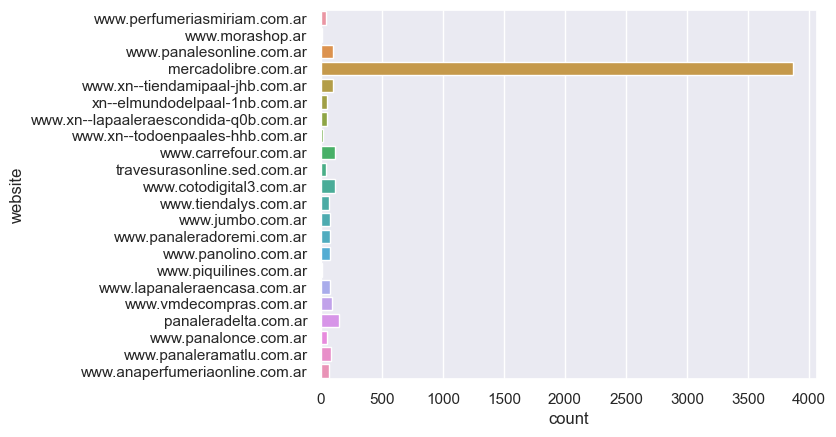
\includegraphics{output_4_0.png}
\caption{png}
\end{figure}

\hypertarget{distribuciuxf3n-items-websites-sin-mercadolibre}{%
\subsubsection{Distribución items websites (sin
Mercadolibre)}\label{distribuciuxf3n-items-websites-sin-mercadolibre}}

Observamos la distribución de los websites quitando Mercadolibre

\begin{Shaded}
\begin{Highlighting}[]
\NormalTok{e }\OperatorTok{=}\NormalTok{ df[df[}\StringTok{\textquotesingle{}website\textquotesingle{}}\NormalTok{] }\OperatorTok{!=} \StringTok{\textquotesingle{}mercadolibre.com.ar\textquotesingle{}}\NormalTok{]}
\NormalTok{ax }\OperatorTok{=}\NormalTok{ sns.countplot(y}\OperatorTok{=}\StringTok{"website"}\NormalTok{, data}\OperatorTok{=}\NormalTok{e, orient}\OperatorTok{=}\StringTok{"h"}\NormalTok{)}
\end{Highlighting}
\end{Shaded}

\begin{figure}
\centering
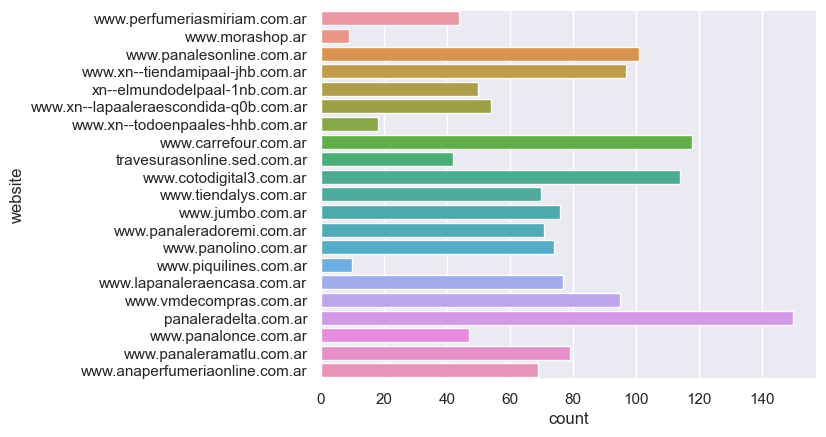
\includegraphics{output_6_0.png}
\caption{png}
\end{figure}

\begin{Shaded}
\begin{Highlighting}[]
\NormalTok{ax }\OperatorTok{=}\NormalTok{ sns.countplot(x}\OperatorTok{=}\StringTok{"brand"}\NormalTok{, data}\OperatorTok{=}\NormalTok{df)}
\NormalTok{add\_values(ax, df)}
\end{Highlighting}
\end{Shaded}

\begin{figure}
\centering
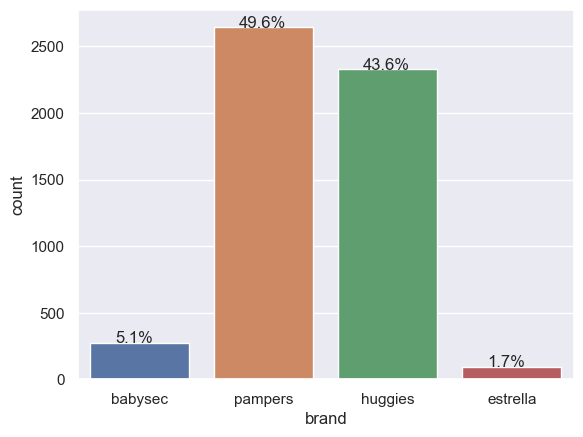
\includegraphics{output_7_0.png}
\caption{png}
\end{figure}

\begin{Shaded}
\begin{Highlighting}[]
\NormalTok{ax }\OperatorTok{=}\NormalTok{ sns.countplot(x}\OperatorTok{=}\StringTok{"size"}\NormalTok{, data}\OperatorTok{=}\NormalTok{df)}
\NormalTok{add\_values(ax, df)}
\end{Highlighting}
\end{Shaded}

\begin{figure}
\centering
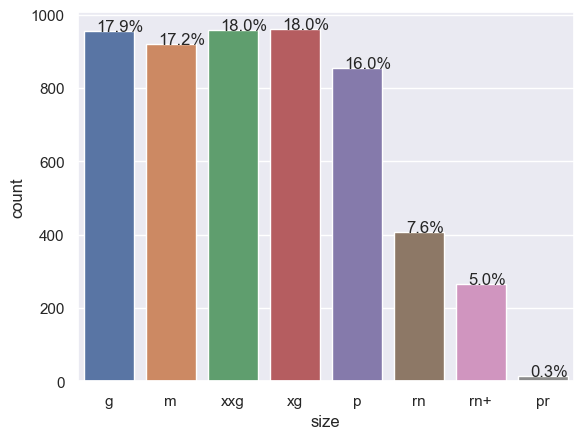
\includegraphics{output_8_0.png}
\caption{png}
\end{figure}

Observamos que a mayor talle mayor precio unitario

\begin{Shaded}
\begin{Highlighting}[]
\NormalTok{order\_sizes }\OperatorTok{=}\NormalTok{ [}\StringTok{"pr"}\NormalTok{, }\StringTok{"rn"}\NormalTok{, }\StringTok{"rn+"}\NormalTok{, }\StringTok{"p"}\NormalTok{, }\StringTok{"m"}\NormalTok{, }\StringTok{"g"}\NormalTok{, }\StringTok{"xg"}\NormalTok{, }\StringTok{"xxg"}\NormalTok{]}
\NormalTok{sns.barplot(data}\OperatorTok{=}\NormalTok{df, x}\OperatorTok{=}\StringTok{"brand"}\NormalTok{, y}\OperatorTok{=}\StringTok{"unit\_price"}\NormalTok{, hue}\OperatorTok{=}\StringTok{"size"}\NormalTok{, hue\_order}\OperatorTok{=}\NormalTok{order\_sizes)}
\end{Highlighting}
\end{Shaded}

\begin{verbatim}
<AxesSubplot: xlabel='brand', ylabel='unit_price'>
\end{verbatim}

\begin{figure}
\centering
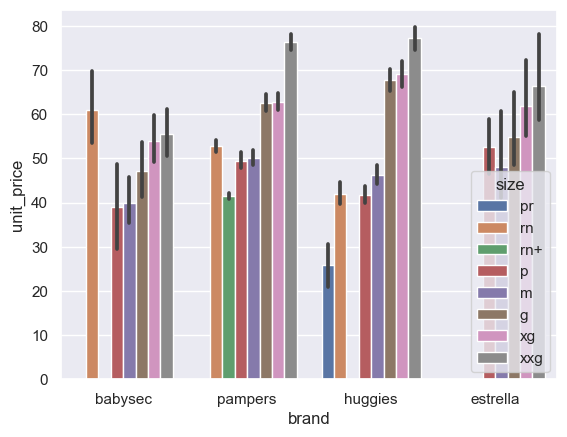
\includegraphics{output_10_1.png}
\caption{png}
\end{figure}

\begin{Shaded}
\begin{Highlighting}[]
\NormalTok{ax }\OperatorTok{=}\NormalTok{ sns.barplot(data}\OperatorTok{=}\NormalTok{df, x}\OperatorTok{=}\StringTok{"brand"}\NormalTok{, y}\OperatorTok{=}\StringTok{"unit\_price"}\NormalTok{)}
\end{Highlighting}
\end{Shaded}

\begin{figure}
\centering
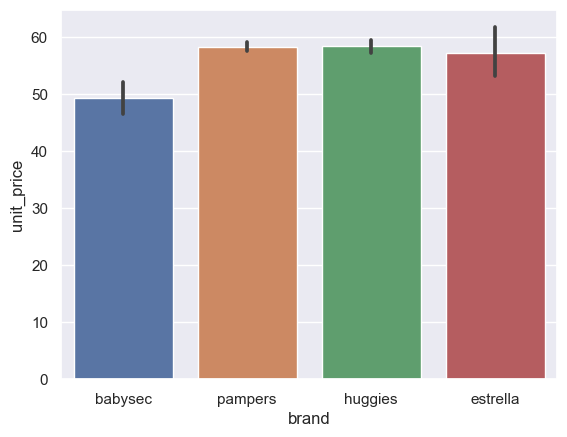
\includegraphics{output_11_0.png}
\caption{png}
\end{figure}

\hypertarget{distribuciones-utilizadas}{%
\subsubsection{Distribuciones
utilizadas}\label{distribuciones-utilizadas}}

Utilizando una distribución normal con 1 unidad desvio standard.
Utilizamos las siguientes configuraciones:

\begin{itemize}
\tightlist
\item
  Recién nacido hasta 2 meses - 7 pañales al dia
\item
  De 3 a 8 meses - 6 pañales al dia
\item
  De 9 a 24 meses - 5 pañales al dia
\end{itemize}

\begin{Shaded}
\begin{Highlighting}[]
\ImportTok{import}\NormalTok{ random}
\NormalTok{\_rand }\OperatorTok{=} \KeywordTok{lambda}\NormalTok{ x: }\BuiltInTok{int}\NormalTok{(random.normalvariate(x, }\DecValTok{1}\NormalTok{))}


\KeywordTok{def}\NormalTok{ \_get\_random\_daily\_usage(month):}
    \ControlFlowTok{if}\NormalTok{ month }\OperatorTok{\textless{}} \DecValTok{3}\NormalTok{:}
        \ControlFlowTok{return}\NormalTok{ \_rand(}\DecValTok{7}\NormalTok{)}
    \ControlFlowTok{if}\NormalTok{ month }\OperatorTok{\textless{}} \DecValTok{9}\NormalTok{:}
        \ControlFlowTok{return}\NormalTok{ \_rand(}\DecValTok{6}\NormalTok{)}
    \ControlFlowTok{return}\NormalTok{ \_rand(}\DecValTok{5}\NormalTok{)}

\NormalTok{plt.hist([\_get\_random\_daily\_usage(}\DecValTok{1}\NormalTok{) }\ControlFlowTok{for}\NormalTok{ \_ }\KeywordTok{in} \BuiltInTok{range}\NormalTok{(}\DecValTok{1\_000\_000}\NormalTok{)], bins}\OperatorTok{=}\DecValTok{100}\NormalTok{)}
\NormalTok{plt.show()}
\end{Highlighting}
\end{Shaded}

\begin{figure}
\centering
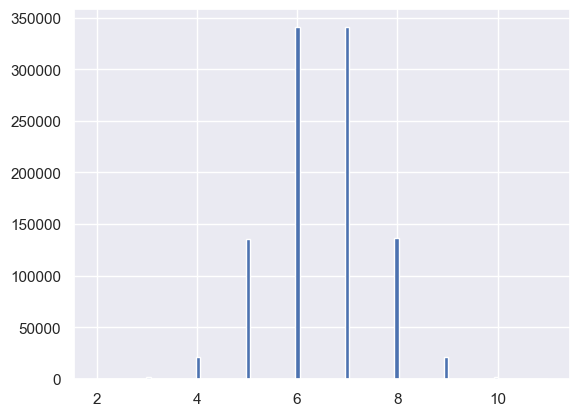
\includegraphics{output_13_0.png}
\caption{png}
\end{figure}

\begin{Shaded}
\begin{Highlighting}[]

\end{Highlighting}
\end{Shaded}

\hypertarget{consumo-de-pauxf1ales-vs-canasta-buxe1sica}{%
\subsection{Consumo de pañales VS canasta
básica}\label{consumo-de-pauxf1ales-vs-canasta-buxe1sica}}

A continuación comparamos el consumo de pañales mensual vs la canasta
básica.

\begin{Shaded}
\begin{Highlighting}[]
\NormalTok{cb }\OperatorTok{=}\NormalTok{ pd.read\_excel(}\StringTok{\textquotesingle{}serie\_cba\_cbt.xls\textquotesingle{}}\NormalTok{)}
\NormalTok{canasta\_basica\_indigencia }\OperatorTok{=}\NormalTok{ cb.loc[}\DecValTok{83}\NormalTok{][}\DecValTok{1}\NormalTok{]}
\NormalTok{canasta\_basica }\OperatorTok{=}\NormalTok{ cb.loc[}\DecValTok{83}\NormalTok{][}\DecValTok{3}\NormalTok{]}
\end{Highlighting}
\end{Shaded}

\begin{Shaded}
\begin{Highlighting}[]
\CommentTok{\# Los primeros 6 Meses de vida, 6 y 12 pañales}

\KeywordTok{def}\NormalTok{ \_cal\_canasta(month):}
\NormalTok{    avg\_daily\_usage }\OperatorTok{=}\NormalTok{ \_get\_random\_daily\_usage(month) }
\NormalTok{    avg\_monthly\_usage }\OperatorTok{=} \DecValTok{30} \OperatorTok{*}\NormalTok{ avg\_daily\_usage}
\NormalTok{    canasta\_basica }\OperatorTok{=}\NormalTok{ cb.loc[}\DecValTok{83}\NormalTok{][}\DecValTok{3}\NormalTok{]}

\NormalTok{    avg\_cost\_diapers }\OperatorTok{=}\NormalTok{ df[}\StringTok{\textquotesingle{}unit\_price\textquotesingle{}}\NormalTok{].mean()  }\OperatorTok{*}\NormalTok{ avg\_monthly\_usage}
    \BuiltInTok{print}\NormalTok{(}\SpecialStringTok{f"Bebe de }\SpecialCharTok{\{}\NormalTok{month}\SpecialCharTok{\}}\SpecialStringTok{ mes/es"}\NormalTok{)}
    \BuiltInTok{print}\NormalTok{(}\SpecialStringTok{f"Consumo promedio diario: }\SpecialCharTok{\{}\NormalTok{avg\_monthly\_usage}\SpecialCharTok{\}}\SpecialStringTok{"}\NormalTok{)}
    \BuiltInTok{print}\NormalTok{(}\SpecialStringTok{f"Costo promedio mensual en pañales: }\SpecialCharTok{\{}\NormalTok{avg\_cost\_diapers}\SpecialCharTok{\}}\SpecialStringTok{"}\NormalTok{)}
    \BuiltInTok{print}\NormalTok{(}\SpecialStringTok{f"Canasta básica mensual {-} Septiembre 2022: }\SpecialCharTok{\{}\NormalTok{canasta\_basica}\SpecialCharTok{\}}\SpecialStringTok{"}\NormalTok{)}
    \BuiltInTok{print}\NormalTok{(}\SpecialStringTok{f"\% de canasta basica: }\SpecialCharTok{\{}\NormalTok{avg\_cost\_diapers }\OperatorTok{/}\NormalTok{ canasta\_basica}\SpecialCharTok{\}}\SpecialStringTok{"}\NormalTok{)}
    \BuiltInTok{print}\NormalTok{(}\StringTok{"}\CharTok{\textbackslash{}n}\StringTok{"}\NormalTok{)}
    
\NormalTok{\_cal\_canasta(}\DecValTok{1}\NormalTok{)}
\NormalTok{\_cal\_canasta(}\DecValTok{6}\NormalTok{)}
\NormalTok{\_cal\_canasta(}\DecValTok{12}\NormalTok{)}
\end{Highlighting}
\end{Shaded}

\begin{verbatim}
Bebe de 1 mes/es
Consumo promedio diario: 180
Costo promedio mensual en pañales: 10405.506466729146
Canasta básica mensual - Septiembre 2022: 41493.24
% de canasta basica: 0.2507759448702764


Bebe de 6 mes/es
Consumo promedio diario: 150
Costo promedio mensual en pañales: 8671.255388940956
Canasta básica mensual - Septiembre 2022: 41493.24
% de canasta basica: 0.20897995405856365


Bebe de 12 mes/es
Consumo promedio diario: 150
Costo promedio mensual en pañales: 8671.255388940956
Canasta básica mensual - Septiembre 2022: 41493.24
% de canasta basica: 0.20897995405856365
\end{verbatim}

\hypertarget{to-do}{%
\subsubsection{TO-DO:}\label{to-do}}

\begin{itemize}
\tightlist
\item
  Agregar una serie de consumo promedio mensual o diario. Evitar funcion
  random creada.
\end{itemize}

\hypertarget{presupuesto-destinado-a-pauxf1ales-en-los-primeros-n-meses-de-vida-del-bebe}{%
\subsection{Presupuesto destinado a pañales en los primeros n meses de
vida del
bebe}\label{presupuesto-destinado-a-pauxf1ales-en-los-primeros-n-meses-de-vida-del-bebe}}

A continuación evaluamos diferentes presupuestos destinados a gastar en
pañales para los primeros 32 meses de vida del bebe. Calculamos
utilizando los percentiles de crecimiento de la OMS para niños y niñas.

\begin{Shaded}
\begin{Highlighting}[]
\NormalTok{bp }\OperatorTok{=}\NormalTok{ pd.read\_csv(}\StringTok{\textquotesingle{}tab\_wfa\_boys\_p\_0\_5.csv\textquotesingle{}}\NormalTok{)}
\NormalTok{gp }\OperatorTok{=}\NormalTok{ pd.read\_csv(}\StringTok{\textquotesingle{}tab\_wfa\_girls\_p\_0\_5.csv\textquotesingle{}}\NormalTok{)}
\NormalTok{bp.head()}
\end{Highlighting}
\end{Shaded}

Month

L

M

S

P01

P1

P3

P5

P10

P15

P25

P50

P75

P85

P90

P95

P97

P99

P999

0

0

0.3487

3.3464

0.14602

2.0

2.3

2.5

2.6

2.8

2.9

3.0

3.3

3.7

3.9

4.0

4.2

4.3

4.6

5.1

1

1

0.2297

4.4709

0.13395

2.9

3.2

3.4

3.6

3.8

3.9

4.1

4.5

4.9

5.1

5.3

5.5

5.7

6.0

6.6

2

2

0.1970

5.5675

0.12385

3.7

4.1

4.4

4.5

4.7

4.9

5.1

5.6

6.0

6.3

6.5

6.8

7.0

7.4

8.1

3

3

0.1738

6.3762

0.11727

4.4

4.8

5.1

5.2

5.5

5.6

5.9

6.4

6.9

7.2

7.4

7.7

7.9

8.3

9.1

4

4

0.1553

7.0023

0.11316

4.9

5.4

5.6

5.8

6.0

6.2

6.5

7.0

7.6

7.9

8.1

8.4

8.6

9.1

9.8

\hypertarget{consumo-mensual-de-pauxf1ales}{%
\subsubsection{Consumo mensual de
pañales}\label{consumo-mensual-de-pauxf1ales}}

Aplicamos a los percenitles de crecimiento la siguiente función que
convierte el peso para ese percentil en cantidad de dinero promedio a
gastar en base a los items que aplican para ese determinado percentil.

Ejemplo: Para el percentil P01 (\emph{P}) en el mes 0 (\emph{m}) tenemos
que el bebe pesará 2.0kg (\emph{Kmp}), entonces buscamos los items en
los que \emph{target\_kg\_min \textless= Kmp \textless= target\_kg\_max}
y calculamos un promedio de todos.

\begin{Shaded}
\begin{Highlighting}[]
\KeywordTok{def}\NormalTok{ \_filter\_series(target\_kg, month):}
    \CommentTok{\# Calculamos el costo mensual promedio para el percentil en base a *target\_kg*}
    \CommentTok{\# Utilizando un consumo mensual fijo de pañales}

\NormalTok{    \_df }\OperatorTok{=}\NormalTok{ df[df[}\StringTok{\textquotesingle{}target\_kg\_min\textquotesingle{}}\NormalTok{] }\OperatorTok{\textless{}=}\NormalTok{ target\_kg]}
\NormalTok{    \_df[target\_kg }\OperatorTok{\textless{}=}\NormalTok{ \_df[}\StringTok{\textquotesingle{}target\_kg\_max\textquotesingle{}}\NormalTok{]]}
    \ControlFlowTok{return}\NormalTok{ \_df[}\StringTok{\textquotesingle{}unit\_price\textquotesingle{}}\NormalTok{].mean() }\OperatorTok{*}\NormalTok{ \_get\_random\_daily\_usage(month) }\OperatorTok{*} \DecValTok{30}

\KeywordTok{def}\NormalTok{ \_filter\_d(target\_kg):}
    \ControlFlowTok{return}\NormalTok{ pd.Series([\_filter\_series(e, i) }\ControlFlowTok{for}\NormalTok{ i, e }\KeywordTok{in} \BuiltInTok{enumerate}\NormalTok{(target\_kg)])}
\end{Highlighting}
\end{Shaded}

\hypertarget{en-niuxf1os}{%
\paragraph{En Niños}\label{en-niuxf1os}}

\begin{Shaded}
\begin{Highlighting}[]
\NormalTok{keys }\OperatorTok{=}\NormalTok{ [ }\StringTok{\textquotesingle{}P01\textquotesingle{}}\NormalTok{, }\StringTok{\textquotesingle{}P1\textquotesingle{}}\NormalTok{, }\StringTok{\textquotesingle{}P3\textquotesingle{}}\NormalTok{, }\StringTok{\textquotesingle{}P5\textquotesingle{}}\NormalTok{, }\StringTok{\textquotesingle{}P10\textquotesingle{}}\NormalTok{, }\StringTok{\textquotesingle{}P15\textquotesingle{}}\NormalTok{, }\StringTok{\textquotesingle{}P25\textquotesingle{}}\NormalTok{, }\StringTok{\textquotesingle{}P50\textquotesingle{}}\NormalTok{, }\StringTok{\textquotesingle{}P75\textquotesingle{}}\NormalTok{, }\StringTok{\textquotesingle{}P85\textquotesingle{}}\NormalTok{, }\StringTok{\textquotesingle{}P90\textquotesingle{}}\NormalTok{, }\StringTok{\textquotesingle{}P95\textquotesingle{}}\NormalTok{, }\StringTok{\textquotesingle{}P97\textquotesingle{}}\NormalTok{, }\StringTok{\textquotesingle{}P99\textquotesingle{}}\NormalTok{,}\StringTok{\textquotesingle{}P999\textquotesingle{}}\NormalTok{]}

\NormalTok{nbp }\OperatorTok{=}\NormalTok{ bp[keys]}
\NormalTok{nbp }\OperatorTok{=}\NormalTok{ nbp.}\BuiltInTok{apply}\NormalTok{(\_filter\_d)}
\NormalTok{nbp.describe()}
\end{Highlighting}
\end{Shaded}

P01

P1

P3

P5

P10

P15

P25

P50

P75

P85

P90

P95

P97

P99

P999

count

33.000000

33.000000

33.000000

33.000000

33.000000

33.000000

33.000000

33.000000

33.000000

33.000000

33.000000

33.000000

33.000000

33.000000

33.000000

mean

6178.014816

6960.683450

6999.539405

6650.105474

7782.385617

7268.743311

7279.457397

7704.717482

7245.891295

7391.635982

7646.187084

7606.424599

7516.025418

7601.732060

8176.590554

std

1676.850010

1930.305967

1742.766060

1339.608590

1317.309776

1792.892398

1761.941151

1565.425599

1409.166941

1740.425950

1616.561115

1678.527337

1960.957164

1973.178162

1533.233906

min

3058.472424

4140.795043

3058.472424

4587.708636

5521.060057

4140.795043

4587.708636

4587.708636

3468.502156

3241.099497

4861.649246

3242.482782

4587.708636

1734.251078

4863.724173

25\%

5193.575575

5521.060057

5521.060057

5524.365066

6901.325071

6116.944848

6116.944848

6484.965564

6123.793915

6123.793915

6484.965564

6482.198995

6116.944848

6937.004311

6937.004311

50\%

5524.365066

6905.456332

6901.325071

6766.346939

7654.742394

7646.181060

7646.181060

7958.904950

7646.181060

7646.181060

7654.742394

7654.742394

7646.181060

8102.748743

8671.255389

75\%

7646.181060

8281.590085

8281.590085

7646.181060

9088.757257

8281.590085

9088.757257

9175.417272

8106.206955

8671.255389

8671.255389

8671.255389

8671.255389

8671.255389

8671.255389

max

9621.558597

10704.653484

10704.653484

9185.690873

10704.653484

10704.653484

10716.639351

9723.298492

10387.151150

10704.653484

12139.757545

10826.155102

12139.757545

11685.545044

11343.848240

\begin{Shaded}
\begin{Highlighting}[]
\NormalTok{keys }\OperatorTok{=}\NormalTok{ [ }\StringTok{\textquotesingle{}P01\textquotesingle{}}\NormalTok{, }\StringTok{\textquotesingle{}P1\textquotesingle{}}\NormalTok{, }\StringTok{\textquotesingle{}P3\textquotesingle{}}\NormalTok{, }\StringTok{\textquotesingle{}P5\textquotesingle{}}\NormalTok{, }\StringTok{\textquotesingle{}P10\textquotesingle{}}\NormalTok{, }\StringTok{\textquotesingle{}P15\textquotesingle{}}\NormalTok{, }\StringTok{\textquotesingle{}P25\textquotesingle{}}\NormalTok{, }\StringTok{\textquotesingle{}P50\textquotesingle{}}\NormalTok{, }\StringTok{\textquotesingle{}P75\textquotesingle{}}\NormalTok{, }\StringTok{\textquotesingle{}P85\textquotesingle{}}\NormalTok{, }\StringTok{\textquotesingle{}P90\textquotesingle{}}\NormalTok{, }\StringTok{\textquotesingle{}P95\textquotesingle{}}\NormalTok{, }\StringTok{\textquotesingle{}P97\textquotesingle{}}\NormalTok{, }\StringTok{\textquotesingle{}P99\textquotesingle{}}\NormalTok{,}\StringTok{\textquotesingle{}P999\textquotesingle{}}\NormalTok{]}

\NormalTok{nbp }\OperatorTok{=}\NormalTok{ bp[keys]}
\NormalTok{nbp }\OperatorTok{=}\NormalTok{ nbp.}\BuiltInTok{apply}\NormalTok{(\_filter\_d)}
\NormalTok{nbp.describe()}
\end{Highlighting}
\end{Shaded}

P01

P1

P3

P5

P10

P15

P25

P50

P75

P85

P90

P95

P97

P99

P999

count

33.000000

33.000000

33.000000

33.000000

33.000000

33.000000

33.000000

33.000000

33.000000

33.000000

33.000000

33.000000

33.000000

33.000000

33.000000

mean

6178.014816

6960.683450

6999.539405

6650.105474

7782.385617

7268.743311

7279.457397

7704.717482

7245.891295

7391.635982

7646.187084

7606.424599

7516.025418

7601.732060

8176.590554

std

1676.850010

1930.305967

1742.766060

1339.608590

1317.309776

1792.892398

1761.941151

1565.425599

1409.166941

1740.425950

1616.561115

1678.527337

1960.957164

1973.178162

1533.233906

min

3058.472424

4140.795043

3058.472424

4587.708636

5521.060057

4140.795043

4587.708636

4587.708636

3468.502156

3241.099497

4861.649246

3242.482782

4587.708636

1734.251078

4863.724173

25\%

5193.575575

5521.060057

5521.060057

5524.365066

6901.325071

6116.944848

6116.944848

6484.965564

6123.793915

6123.793915

6484.965564

6482.198995

6116.944848

6937.004311

6937.004311

50\%

5524.365066

6905.456332

6901.325071

6766.346939

7654.742394

7646.181060

7646.181060

7958.904950

7646.181060

7646.181060

7654.742394

7654.742394

7646.181060

8102.748743

8671.255389

75\%

7646.181060

8281.590085

8281.590085

7646.181060

9088.757257

8281.590085

9088.757257

9175.417272

8106.206955

8671.255389

8671.255389

8671.255389

8671.255389

8671.255389

8671.255389

max

9621.558597

10704.653484

10704.653484

9185.690873

10704.653484

10704.653484

10716.639351

9723.298492

10387.151150

10704.653484

12139.757545

10826.155102

12139.757545

11685.545044

11343.848240

\begin{Shaded}
\begin{Highlighting}[]
\CommentTok{\# Solo los primeros 6 Meses de Vida}
\NormalTok{nbp.iloc[[}\DecValTok{0}\NormalTok{, }\DecValTok{1}\NormalTok{, }\DecValTok{2}\NormalTok{, }\DecValTok{3}\NormalTok{, }\DecValTok{4}\NormalTok{, }\DecValTok{5}\NormalTok{, }\DecValTok{6}\NormalTok{]].describe()}
\end{Highlighting}
\end{Shaded}

P01

P1

P3

P5

P10

P15

P25

P50

P75

P85

P90

P95

P97

P99

P999

count

7.000000

7.000000

7.000000

7.000000

7.000000

7.000000

7.000000

7.000000

7.000000

7.000000

7.000000

7.000000

7.000000

7.000000

7.000000

mean

7840.435126

8241.731583

7119.900116

7110.552761

8693.012494

7891.771377

8481.169242

8528.699931

8303.922867

8570.611333

7909.341994

8020.298859

8198.534524

8735.295127

8688.593936

std

1574.805937

1700.245871

1371.275526

1449.639767

768.725706

2020.067941

1182.867952

1035.569603

1216.572411

1542.811940

1083.772612

1681.593109

1659.378744

1530.397646

1501.987622

min

5193.575575

5193.575575

5377.095292

5377.095292

7790.363363

4140.795043

6901.325071

6766.346939

6901.325071

5521.060057

6901.325071

5521.060057

5521.060057

6901.325071

6116.944848

25\%

7141.166416

7420.492721

6196.800956

6006.514763

8183.333276

7345.844217

7510.470699

8120.247518

7593.523209

8035.976724

6903.390701

7273.753065

7275.818696

7963.885573

7968.166240

50\%

8065.642938

9088.757257

6901.325071

6766.346939

8281.590085

8119.616327

9088.757257

8281.590085

8281.590085

9409.916761

7790.363363

7790.363363

8281.590085

8281.590085

9175.417272

75\%

8859.967970

9453.473853

8039.260639

8264.320156

9375.306178

8951.574341

9347.652935

9375.306178

8685.173671

9661.855100

8728.503678

8728.503678

9324.151493

9175.417272

9418.636186

max

9621.558597

9661.855100

9088.757257

9088.757257

9661.855100

10387.151150

9661.855100

9661.855100

10387.151150

9667.638865

9409.916761

10826.155102

10387.151150

11685.545044

10754.190584

\hypertarget{en-niuxf1as}{%
\paragraph{En Niñas}\label{en-niuxf1as}}

\begin{Shaded}
\begin{Highlighting}[]
\NormalTok{ngp }\OperatorTok{=}\NormalTok{ gp[keys]}
\NormalTok{ngp }\OperatorTok{=}\NormalTok{ ngp.}\BuiltInTok{apply}\NormalTok{(\_filter\_d)}
\NormalTok{ngp.describe()}
\end{Highlighting}
\end{Shaded}

P01

P1

P3

P5

P10

P15

P25

P50

P75

P85

P90

P95

P97

P99

P999

count

33.000000

33.000000

33.000000

33.000000

33.000000

33.000000

33.000000

33.000000

33.000000

33.000000

33.000000

33.000000

33.000000

33.000000

33.000000

mean

6139.929261

6495.208332

6872.573437

6825.106890

7235.769702

6845.927743

7517.419314

7327.951676

7326.780744

7312.386197

7570.865992

7331.357812

7574.374486

7436.382652

7441.569069

std

1582.139851

1611.102284

1735.786575

1603.357776

1946.359243

1454.994569

1395.017348

1426.215891

1621.468760

1593.858086

1676.892008

1984.271179

1576.282304

1977.728034

1757.097397

min

2760.530028

2760.530028

4140.795043

4140.795043

3058.472424

4587.708636

5521.060057

4140.795043

4587.708636

3241.099497

4592.845436

4592.845436

5202.753233

3468.502156

4861.649246

25\%

5521.060057

5521.060057

5521.060057

5524.365066

6116.944848

5524.365066

6491.969469

6482.198995

6482.198995

6484.965564

6482.198995

5202.753233

6482.198995

6123.793915

6484.965564

50\%

5524.365066

6721.369115

6901.325071

6721.369115

6901.325071

6901.325071

7646.181060

7646.181060

6905.456332

7646.181060

7646.181060

6937.004311

6937.004311

7646.181060

6937.004311

75\%

6901.325071

6905.456332

8065.642938

7646.181060

8286.547598

7654.742394

8281.590085

8102.748743

8106.206955

8281.590085

8281.590085

9175.417272

8671.255389

8671.255389

8671.255389

max

9621.558597

9472.885714

10387.151150

10996.066968

11685.545044

9661.855100

10826.155102

9727.448346

10704.653484

10405.506467

11348.689737

10704.653484

12139.757545

10826.155102

12233.889696

\begin{Shaded}
\begin{Highlighting}[]
\CommentTok{\# Solo los primeros 6 Meses de Vida}
\NormalTok{ngp.iloc[[}\DecValTok{0}\NormalTok{, }\DecValTok{1}\NormalTok{, }\DecValTok{2}\NormalTok{, }\DecValTok{3}\NormalTok{, }\DecValTok{4}\NormalTok{, }\DecValTok{5}\NormalTok{, }\DecValTok{6}\NormalTok{]].describe()}
\end{Highlighting}
\end{Shaded}

P01

P1

P3

P5

P10

P15

P25

P50

P75

P85

P90

P95

P97

P99

P999

count

7.000000

7.000000

7.000000

7.000000

7.000000

7.000000

7.000000

7.000000

7.000000

7.000000

7.000000

7.000000

7.000000

7.000000

7.000000

mean

7617.291558

7198.044687

7996.608608

8039.745651

8795.489293

8075.299648

8276.103528

8098.317250

7928.759125

7329.377620

8587.566842

8767.674013

8494.565939

8208.602066

7960.968465

std

1566.631721

1830.530246

1975.376740

1935.781089

2163.474174

1066.776743

1656.492167

1267.459734

1271.953723

1222.315104

1423.389045

782.173178

1212.167054

1541.538148

2097.916048

min

5193.575575

4059.808163

5413.077551

5413.077551

6766.346939

6766.346939

6491.969469

6632.420792

6491.969469

5521.060057

6491.969469

7790.363363

6901.325071

6491.969469

6116.944848

25\%

6682.255662

6491.969469

6601.720457

6606.669292

6833.836005

7331.452609

6811.347093

6901.325071

6901.325071

6696.647270

8173.616512

8281.590085

7483.484004

7273.753065

6511.200590

50\%

7790.363363

6721.369115

8065.642938

8281.590085

8065.642938

8065.642938

8281.590085

8281.590085

7790.363363

6901.325071

8281.590085

8286.547598

9088.757257

7646.181060

7790.363363

75\%

8675.516023

8667.903741

9453.473853

9187.073183

10691.609059

8685.173671

9355.157927

9249.337009

8877.237900

8200.603206

8971.722592

9535.885930

9418.636186

8974.201349

8281.590085

max

9621.558597

9285.389109

10387.151150

10996.066968

11685.545044

9661.855100

10826.155102

9472.885714

9661.855100

9088.757257

11048.730131

9661.855100

9667.638865

10826.155102

12233.889696

\hypertarget{comparativa---niuxf1os-vs-niuxf1as}{%
\paragraph{Comparativa - Niños vs
Niñas}\label{comparativa---niuxf1os-vs-niuxf1as}}

\begin{Shaded}
\begin{Highlighting}[]
\NormalTok{fig, ax }\OperatorTok{=}\NormalTok{plt.subplots(}\DecValTok{1}\NormalTok{,}\DecValTok{2}\NormalTok{, figsize}\OperatorTok{=}\NormalTok{(}\DecValTok{14}\NormalTok{, }\DecValTok{7}\NormalTok{))}
\NormalTok{b }\OperatorTok{=}\NormalTok{ sns.barplot(data}\OperatorTok{=}\NormalTok{nbp, ax}\OperatorTok{=}\NormalTok{ax[}\DecValTok{0}\NormalTok{])}
\NormalTok{b.set\_xlabel(}\StringTok{"Percentil"}\NormalTok{)}
\NormalTok{b.set\_ylabel(}\StringTok{"Monthly Cost"}\NormalTok{)}
\CommentTok{\# b.set\_ylim(12000)}
\NormalTok{b.set\_title(}\StringTok{"Boys"}\NormalTok{)}

\NormalTok{g }\OperatorTok{=}\NormalTok{ sns.barplot(data}\OperatorTok{=}\NormalTok{ngp, ax}\OperatorTok{=}\NormalTok{ax[}\DecValTok{1}\NormalTok{])}
\NormalTok{g.set\_xlabel(}\StringTok{"Percentil"}\NormalTok{)}
\NormalTok{g.set\_ylabel(}\StringTok{"Monthly Cost"}\NormalTok{)}
\CommentTok{\# g.set\_ylim(12000)}
\NormalTok{g.set\_title(}\StringTok{"Girls"}\NormalTok{)}
\end{Highlighting}
\end{Shaded}

\begin{verbatim}
Text(0.5, 1.0, 'Girls')
\end{verbatim}

\begin{figure}
\centering
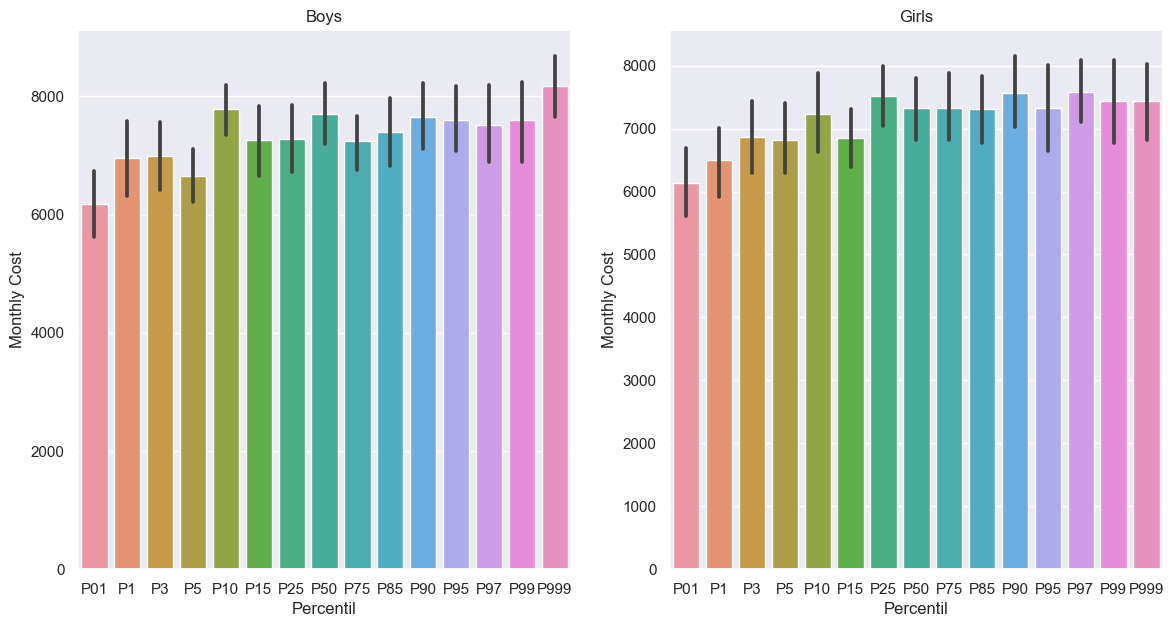
\includegraphics{output_31_1.png}
\caption{png}
\end{figure}

\begin{Shaded}
\begin{Highlighting}[]
\NormalTok{fig, ax }\OperatorTok{=}\NormalTok{ plt.subplots(}\DecValTok{1}\NormalTok{,}\DecValTok{2}\NormalTok{, figsize}\OperatorTok{=}\NormalTok{(}\DecValTok{14}\NormalTok{, }\DecValTok{7}\NormalTok{))}

\NormalTok{b }\OperatorTok{=}\NormalTok{ sns.boxplot(data}\OperatorTok{=}\NormalTok{nbp, ax}\OperatorTok{=}\NormalTok{ax[}\DecValTok{0}\NormalTok{])}
\NormalTok{b.set\_xlabel(}\StringTok{"Percentil"}\NormalTok{)}
\NormalTok{b.set\_ylabel(}\StringTok{"Monthly Cost"}\NormalTok{)}
\NormalTok{b.set\_title(}\StringTok{"Boys"}\NormalTok{)}

\NormalTok{g }\OperatorTok{=}\NormalTok{ sns.boxplot(data}\OperatorTok{=}\NormalTok{ngp, ax}\OperatorTok{=}\NormalTok{ax[}\DecValTok{1}\NormalTok{])}
\NormalTok{g.set\_xlabel(}\StringTok{"Percentil"}\NormalTok{)}
\NormalTok{g.set\_ylabel(}\StringTok{"Monthly Cost"}\NormalTok{)}
\NormalTok{g.set\_title(}\StringTok{"Girls"}\NormalTok{)}
\end{Highlighting}
\end{Shaded}

\begin{verbatim}
Text(0.5, 1.0, 'Girls')
\end{verbatim}

\begin{figure}
\centering
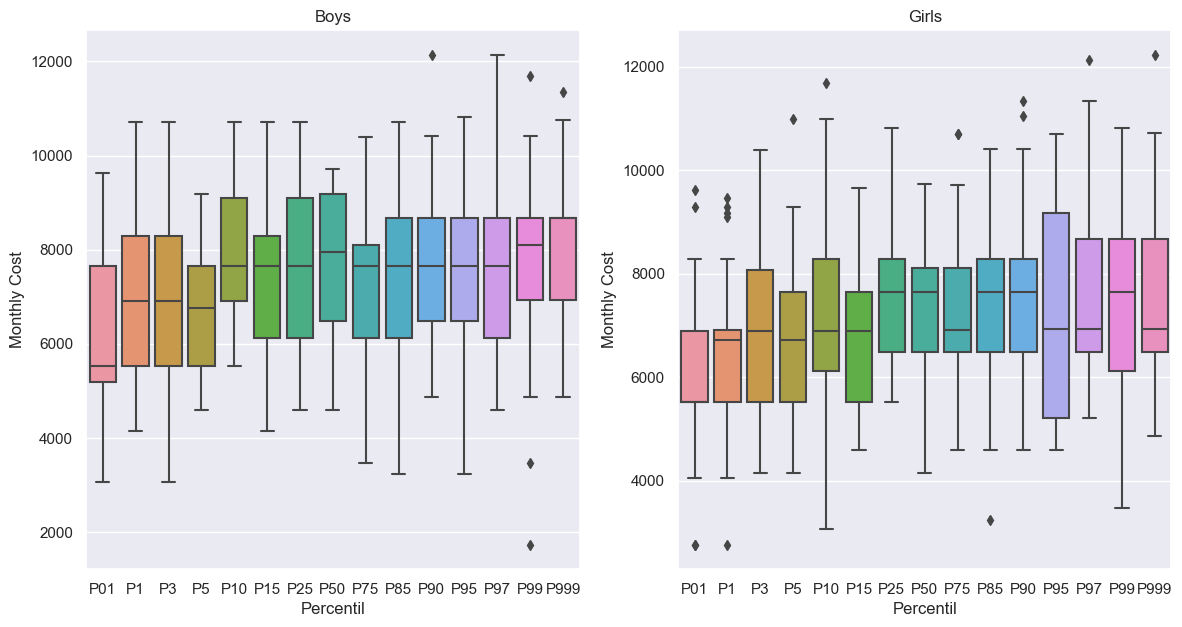
\includegraphics{output_32_1.png}
\caption{png}
\end{figure}

\begin{Shaded}
\begin{Highlighting}[]
\NormalTok{b }\OperatorTok{=}\NormalTok{ sns.displot(data}\OperatorTok{=}\NormalTok{nbp,multiple}\OperatorTok{=}\StringTok{"stack"}\NormalTok{, kind}\OperatorTok{=}\StringTok{"kde"}\NormalTok{,)}
\NormalTok{b.fig.suptitle(}\StringTok{\textquotesingle{}Boys\textquotesingle{}}\NormalTok{)}

\NormalTok{g }\OperatorTok{=}\NormalTok{ sns.displot(data}\OperatorTok{=}\NormalTok{ngp,multiple}\OperatorTok{=}\StringTok{"stack"}\NormalTok{, kind}\OperatorTok{=}\StringTok{"kde"}\NormalTok{)}
\NormalTok{g.fig.suptitle(}\StringTok{\textquotesingle{}Girls\textquotesingle{}}\NormalTok{)}
\end{Highlighting}
\end{Shaded}

\begin{verbatim}
Text(0.5, 0.98, 'Girls')
\end{verbatim}

\begin{figure}
\centering
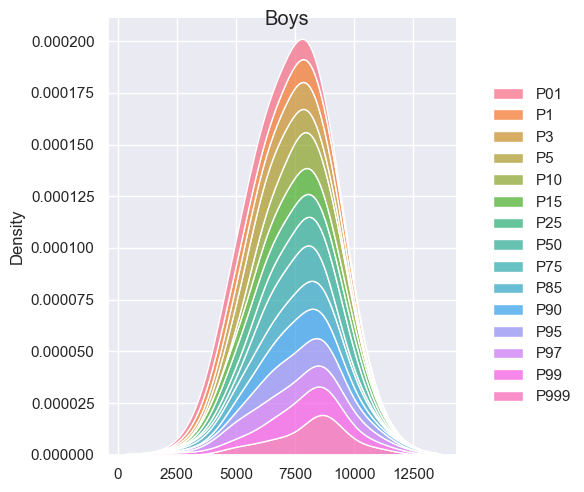
\includegraphics{output_33_1.png}
\caption{png}
\end{figure}

\begin{figure}
\centering
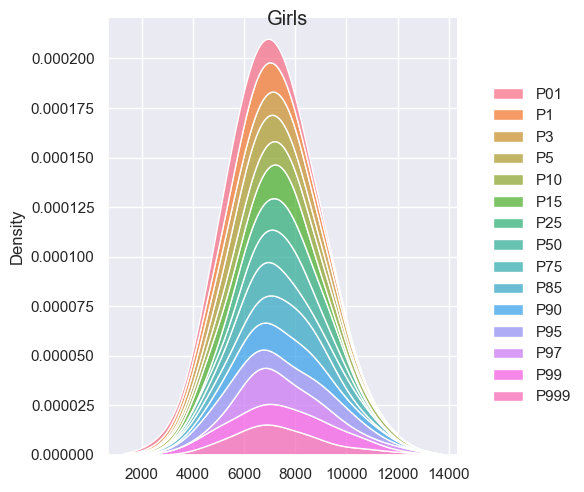
\includegraphics{output_33_2.png}
\caption{png}
\end{figure}

\begin{Shaded}
\begin{Highlighting}[]
\NormalTok{keys }\OperatorTok{=}\NormalTok{ [}
 \StringTok{\textquotesingle{}P01\textquotesingle{}}\NormalTok{,}
 \StringTok{\textquotesingle{}P10\textquotesingle{}}\NormalTok{,}
 \StringTok{\textquotesingle{}P50\textquotesingle{}}\NormalTok{,}
 \StringTok{\textquotesingle{}P85\textquotesingle{}}\NormalTok{,}
 \StringTok{\textquotesingle{}P999\textquotesingle{}}
\NormalTok{]}
\NormalTok{\_nbp }\OperatorTok{=}\NormalTok{ nbp[keys]}
\NormalTok{b }\OperatorTok{=}\NormalTok{ sns.displot(data}\OperatorTok{=}\NormalTok{\_nbp, multiple}\OperatorTok{=}\StringTok{"stack"}\NormalTok{, kind}\OperatorTok{=}\StringTok{"kde"}\NormalTok{)}
\NormalTok{b.fig.suptitle(}\StringTok{\textquotesingle{}Boys\textquotesingle{}}\NormalTok{)}

\NormalTok{\_ngp }\OperatorTok{=}\NormalTok{ ngp[keys]}
\NormalTok{g }\OperatorTok{=}\NormalTok{ sns.displot(data}\OperatorTok{=}\NormalTok{\_ngp, multiple}\OperatorTok{=}\StringTok{"stack"}\NormalTok{, kind}\OperatorTok{=}\StringTok{"kde"}\NormalTok{)}
\NormalTok{g.fig.suptitle(}\StringTok{\textquotesingle{}Girls\textquotesingle{}}\NormalTok{)}
\end{Highlighting}
\end{Shaded}

\begin{verbatim}
Text(0.5, 0.98, 'Girls')
\end{verbatim}

\begin{figure}
\centering
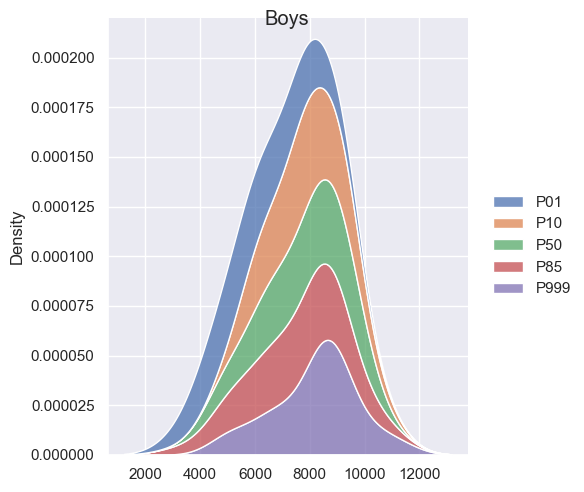
\includegraphics{output_34_1.png}
\caption{png}
\end{figure}

\begin{figure}
\centering
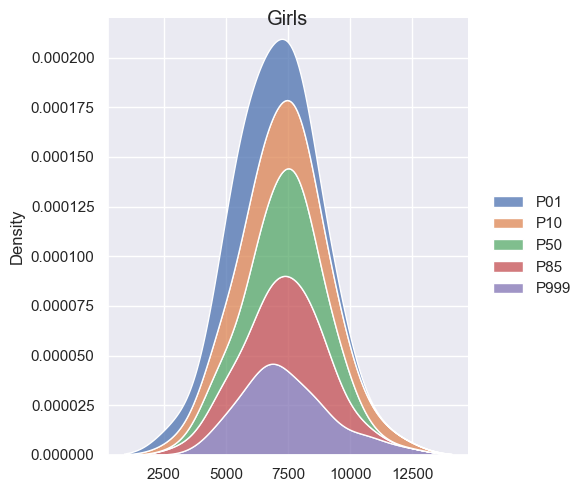
\includegraphics{output_34_2.png}
\caption{png}
\end{figure}

\hypertarget{conclusiones-preliminares}{%
\paragraph{Conclusiones preliminares:}\label{conclusiones-preliminares}}

\begin{itemize}
\tightlist
\item
  Observarmos que hay una tendencia levemente que indica mayor gasto en
  niños, se debe principalmente a que el niño tiene un peso mayor.
\item
  Observamos una distinción entre los percentiles para los siguientes
  percentiles
  \texttt{{[}\ \textquotesingle{}P01\textquotesingle{},\ \textquotesingle{}P10\textquotesingle{},\ \textquotesingle{}P85\textquotesingle{},\ \textquotesingle{}P999\textquotesingle{}\ {]}}
  tanto para niños como niñas.
\item
  La cantidad destinada al gasto de pañales no disminuye, por mas que el
  bebe tienda a utilizar menor cantidad.
\end{itemize}

\hypertarget{comparativa-entre-marcas}{%
\paragraph{Comparativa entre marcas}\label{comparativa-entre-marcas}}

A continuación realizamos el mismo procesamiento pero en lugar de
diferencias el presupuesto por genero, armamos el presupuesto mes a mes
por marca.

\begin{Shaded}
\begin{Highlighting}[]
\KeywordTok{def}\NormalTok{ \_filter\_series(target\_kg, custom\_df, month):}
    \CommentTok{\# Calculamos el costo mensual promedio para el percentil en base a *target\_kg*}
    \CommentTok{\# Utilizando un consumo mensual fijo de pañales}
\NormalTok{    \_df }\OperatorTok{=}\NormalTok{ custom\_df[custom\_df[}\StringTok{\textquotesingle{}target\_kg\_min\textquotesingle{}}\NormalTok{] }\OperatorTok{\textless{}=}\NormalTok{ target\_kg]}
\NormalTok{    \_df[target\_kg }\OperatorTok{\textless{}=}\NormalTok{ \_df[}\StringTok{\textquotesingle{}target\_kg\_max\textquotesingle{}}\NormalTok{]]}
    \ControlFlowTok{return}\NormalTok{ \_df[}\StringTok{\textquotesingle{}unit\_price\textquotesingle{}}\NormalTok{].mean() }\OperatorTok{*}\NormalTok{ \_get\_random\_daily\_usage(month) }\OperatorTok{*} \DecValTok{30}

\KeywordTok{def}\NormalTok{ \_filter\_d(target\_kg, custom\_df):}
    \ControlFlowTok{return}\NormalTok{ pd.Series([\_filter\_series(e, custom\_df, i) }\ControlFlowTok{for}\NormalTok{ i, e }\KeywordTok{in} \BuiltInTok{enumerate}\NormalTok{(target\_kg)])}


\KeywordTok{def}\NormalTok{ \_filter\_brand(brand):}
\NormalTok{    df }\OperatorTok{=}\NormalTok{ prepare\_df()}
    \ControlFlowTok{return}\NormalTok{ df[df[}\StringTok{\textquotesingle{}brand\textquotesingle{}}\NormalTok{] }\OperatorTok{==}\NormalTok{ brand]}

\KeywordTok{def}\NormalTok{ \_prepare\_percentils(brand):}
\NormalTok{    df }\OperatorTok{=}\NormalTok{ \_filter\_brand(brand)}
\NormalTok{    keys }\OperatorTok{=}\NormalTok{ [ }\StringTok{\textquotesingle{}P01\textquotesingle{}}\NormalTok{, }\StringTok{\textquotesingle{}P1\textquotesingle{}}\NormalTok{, }\StringTok{\textquotesingle{}P3\textquotesingle{}}\NormalTok{, }\StringTok{\textquotesingle{}P5\textquotesingle{}}\NormalTok{, }\StringTok{\textquotesingle{}P10\textquotesingle{}}\NormalTok{, }\StringTok{\textquotesingle{}P15\textquotesingle{}}\NormalTok{, }\StringTok{\textquotesingle{}P25\textquotesingle{}}\NormalTok{, }\StringTok{\textquotesingle{}P50\textquotesingle{}}\NormalTok{, }\StringTok{\textquotesingle{}P75\textquotesingle{}}\NormalTok{, }\StringTok{\textquotesingle{}P85\textquotesingle{}}\NormalTok{, }\StringTok{\textquotesingle{}P90\textquotesingle{}}\NormalTok{, }\StringTok{\textquotesingle{}P95\textquotesingle{}}\NormalTok{, }\StringTok{\textquotesingle{}P97\textquotesingle{}}\NormalTok{, }\StringTok{\textquotesingle{}P99\textquotesingle{}}\NormalTok{,}\StringTok{\textquotesingle{}P999\textquotesingle{}}\NormalTok{]}
\NormalTok{    nbp }\OperatorTok{=}\NormalTok{ bp[keys]}
    \ControlFlowTok{return}\NormalTok{ nbp.}\BuiltInTok{apply}\NormalTok{(\_filter\_d, args}\OperatorTok{=}\NormalTok{(df,))}

\NormalTok{h\_df }\OperatorTok{=}\NormalTok{ \_prepare\_percentils(}\StringTok{\textquotesingle{}huggies\textquotesingle{}}\NormalTok{)}
\NormalTok{p\_df }\OperatorTok{=}\NormalTok{ \_prepare\_percentils(}\StringTok{\textquotesingle{}pampers\textquotesingle{}}\NormalTok{)}
\NormalTok{b\_df }\OperatorTok{=}\NormalTok{ \_prepare\_percentils(}\StringTok{\textquotesingle{}babysec\textquotesingle{}}\NormalTok{)}
\NormalTok{e\_df }\OperatorTok{=}\NormalTok{ \_prepare\_percentils(}\StringTok{\textquotesingle{}estrella\textquotesingle{}}\NormalTok{)}
\end{Highlighting}
\end{Shaded}

\begin{Shaded}
\begin{Highlighting}[]
\KeywordTok{def}\NormalTok{ \_add\_fig(df, name, ax):}
\NormalTok{    a }\OperatorTok{=}\NormalTok{ sns.barplot(data}\OperatorTok{=}\NormalTok{df, ax}\OperatorTok{=}\NormalTok{ax)}
\NormalTok{    a.set\_title(name, fontweight}\OperatorTok{=}\StringTok{\textquotesingle{}bold\textquotesingle{}}\NormalTok{)}
\NormalTok{    a.set\_ylabel(}\StringTok{"Monthly Cost"}\NormalTok{)}
\NormalTok{    a.set\_xlabel(}\StringTok{"Percentil"}\NormalTok{)}
    \CommentTok{\# a.set\_ylim(11000)}


\NormalTok{fig, ax }\OperatorTok{=}\NormalTok{plt.subplots(}\DecValTok{1}\NormalTok{,}\DecValTok{2}\NormalTok{, figsize}\OperatorTok{=}\NormalTok{(}\DecValTok{14}\NormalTok{, }\DecValTok{7}\NormalTok{))}
\NormalTok{\_add\_fig(h\_df, }\StringTok{"Huggies"}\NormalTok{, ax}\OperatorTok{=}\NormalTok{ax[}\DecValTok{0}\NormalTok{])}
\NormalTok{\_add\_fig(p\_df, }\StringTok{"Pampers"}\NormalTok{, ax}\OperatorTok{=}\NormalTok{ax[}\DecValTok{1}\NormalTok{])}
\end{Highlighting}
\end{Shaded}

\begin{figure}
\centering
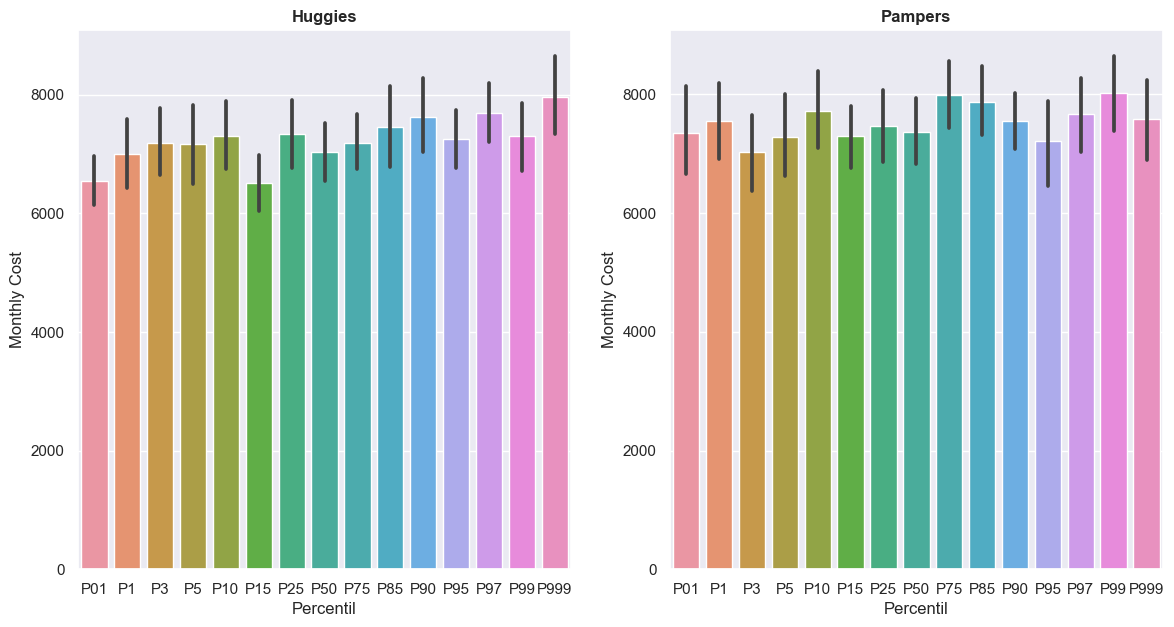
\includegraphics{output_38_0.png}
\caption{png}
\end{figure}

\begin{Shaded}
\begin{Highlighting}[]
\KeywordTok{def}\NormalTok{ \_add\_fig(df, name, ax):}
\NormalTok{    a }\OperatorTok{=}\NormalTok{ sns.boxplot(data}\OperatorTok{=}\NormalTok{df, ax}\OperatorTok{=}\NormalTok{ax)}
\NormalTok{    a.set\_title(name, fontweight}\OperatorTok{=}\StringTok{\textquotesingle{}bold\textquotesingle{}}\NormalTok{)}
\NormalTok{    a.set\_ylabel(}\StringTok{"Monthly Cost"}\NormalTok{)}
\NormalTok{    a.set\_xlabel(}\StringTok{"Percentil"}\NormalTok{)}


\NormalTok{fig, ax }\OperatorTok{=}\NormalTok{plt.subplots(}\DecValTok{1}\NormalTok{,}\DecValTok{2}\NormalTok{, figsize}\OperatorTok{=}\NormalTok{(}\DecValTok{14}\NormalTok{, }\DecValTok{7}\NormalTok{))}
\NormalTok{\_add\_fig(h\_df, }\StringTok{"Huggies"}\NormalTok{, ax}\OperatorTok{=}\NormalTok{ax[}\DecValTok{0}\NormalTok{])}
\NormalTok{\_add\_fig(p\_df, }\StringTok{"Pampers"}\NormalTok{, ax}\OperatorTok{=}\NormalTok{ax[}\DecValTok{1}\NormalTok{])}
\end{Highlighting}
\end{Shaded}

\begin{figure}
\centering
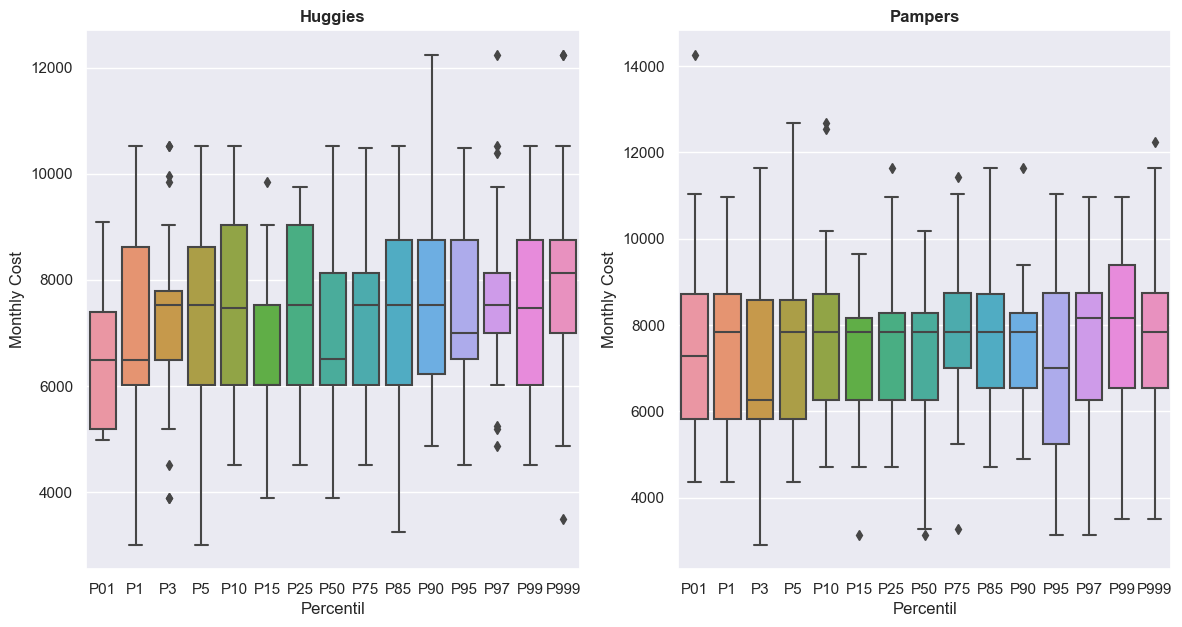
\includegraphics{output_39_0.png}
\caption{png}
\end{figure}

\begin{Shaded}
\begin{Highlighting}[]
\KeywordTok{def}\NormalTok{ \_add\_fig(df, name):}
\NormalTok{    b }\OperatorTok{=}\NormalTok{ sns.displot(data}\OperatorTok{=}\NormalTok{df, multiple}\OperatorTok{=}\StringTok{"stack"}\NormalTok{, kind}\OperatorTok{=}\StringTok{"kde"}\NormalTok{)}
\NormalTok{    b.fig.suptitle(name)}

\NormalTok{\_add\_fig(h\_df, }\StringTok{"Huggies"}\NormalTok{)}
\NormalTok{\_add\_fig(p\_df, }\StringTok{"Pampers"}\NormalTok{)}
\end{Highlighting}
\end{Shaded}

\begin{figure}
\centering
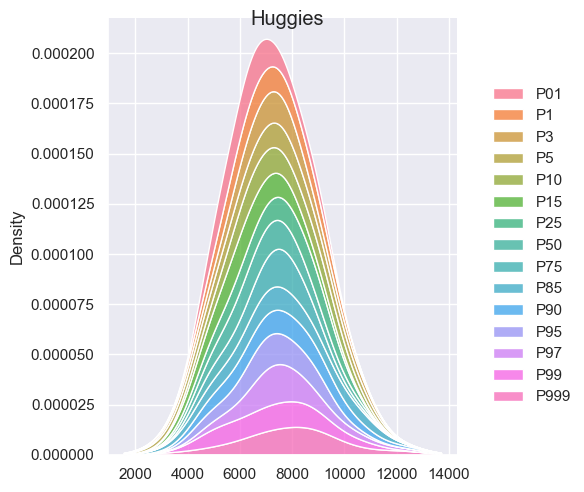
\includegraphics{output_40_0.png}
\caption{png}
\end{figure}

\begin{figure}
\centering
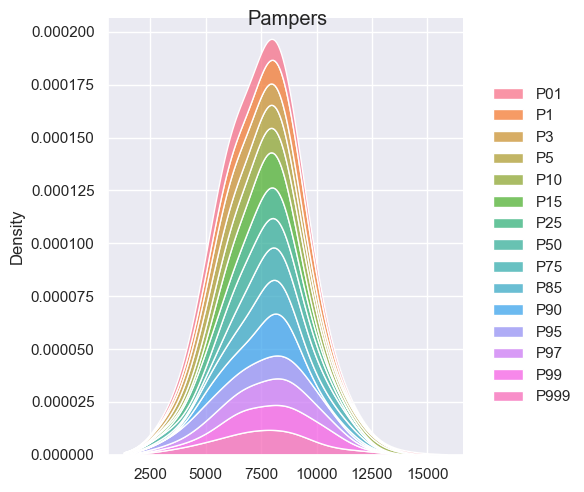
\includegraphics{output_40_1.png}
\caption{png}
\end{figure}

\hypertarget{conclusiones-preliminares-1}{%
\paragraph{Conclusiones
preliminares:}\label{conclusiones-preliminares-1}}

\begin{itemize}
\tightlist
\item
  Pampers (49\%) y Huggies (43.6\%) son las marcas predominantes
  abarcando el \textasciitilde92.6\% de la muestra. Para el caso
  deBabysec y Estrella no podemos garantizar que sean numeros
  representativos porque no llegan al 10\% de la muestra de items.
\item
  Pampers es mas caro que Huggies para talles de pequeños (rn, p, m) que
  corresponden a los percentiles P01 a P15.
\item
\end{itemize}

\end{document}
